\documentclass{rapport}
\usepackage[utf8]{inputenc}

\usepackage{pifont} % Pour les symboles appelés par la macro \ding
\usepackage{url} % Comme son nom l'indique, pour les url...

\usetikzlibrary{positioning} % Bibliothèque tikz pour positionner des nœuds relativement à d'autres

\usepackage[colorlinks, citecolor=red!60!green, linkcolor=blue!60!green, urlcolor=magenta]{hyperref} % Pour que les liens soient cliquables. Les options permettent de mettre les liens en couleur.

\usepackage{algorithm}
\usepackage{algo}
\usepackage{colorationSyntaxique}
\usepackage{amsmath}
\usepackage{diagbox}
\usepackage{graphicx}
\usepackage{listings}
\lstset{                  % Specify language
    basicstyle=\ttfamily\small,     % Code font and size
    keywordstyle=\color{blue},      % Color for keywords
    commentstyle=\color{gray},      % Color for comments
    stringstyle=\color{red},        % Color for strings
    numbers=left,                   % Add line numbers
    numberstyle=\tiny\color{gray},  % Style for line numbers
    % frame=single,                   % Add a border around code
    breaklines=true,                % Line wrapping
    % backgroundcolor=\color{gray!10} % Light gray background
}
% Pour un rapport en français 
\usepackage[french]{babel} % Commenter pour un rapport en anglais
\renewcommand\bibsection{\section*{Bibliographie}} % Commenter pour un rapport en anglais

% \englishTitlePage % Décommenter pour une page de titre en anglais

\pagestyle{fancy}
\renewcommand{\sectionmark}[1]{\markboth{\thesection.\ #1}{}}
\fancyfoot{}

\fancyhead[LE]{\textsl{\leftmark}}
\fancyhead[RE, LO]{\textbf{\thepage}}
\fancyhead[RO]{\textsl{\rightmark}}

\def\Latex{\LaTeX\xspace}
\def\etc{\textit{etc.}\xspace}



\title{Placement des threads sur les cœurs: Threads affinity}
\author{Mehdi Mansour}
\supervisor{Professeur Sid Touati}
\date{Premier semestre de l'année 2024-2025}

%\universityname{Université Côte d'Azur} % Nom de l'université.
\type{TP3} % Type de document
% \formation{Master Informatique} % Nom de la formation

% Retrouver les autres options possibles dans le document rapport.pdf

\begin{document}

  \maketitle

  \begin{abstract}
    Ce rapport a pour objectif de détailler les différents résultats obtenus lors de ce TP3 disponible dans l'archive, nommé «Affinity.pdf».
     \end{abstract}
    %\newcommand{\ppc}{programmation par contraintes\xspace}
\subsection*{Architecture utilisée pour ce TP}
     \noindent
    CPU name:	Intel(R) Core(TM) i7-10700F CPU @ 2.90GHz
    \newline
    CPU type:	Intel Cometlake processor
    \newline
    CPU stepping:	5
    \newline
    \newline
    \noindent
    Hardware Thread Topology
    \newline
    \newline
    Sockets:		1
    \newline
    Cores per socket:	8
    \newline
    Threads per core:	2
    \newline
    Socket 0:		( 0 8 1 9 2 10 3 11 4 12 5 13 6 14 7 15 )
    \newline
    \newline
    NUMA domains:		1
    \newline
    Domain:			0
    \newline
    Processors:		( 0 8 1 9 2 10 3 11 4 12 5 13 6 14 7 15 )
    \newline
    Distances:		10
    \newline
    Free memory:		21746.9 MB
    \newline
    Total memory:		31991.4 MB
    \newline

\subsection*{Topologie du PC}
    \begin{table}[h!]
    \centering
    \begin{tabular}{|c|c|c|c|c|c|c|c|c|}
        \hline
        \multicolumn{9}{|c|}{Topologie graphique} \\
        \hline
        Core & \enspace0\enspace\enspace8 &\enspace1\enspace\enspace9 &\enspace2\enspace\enspace10 &\enspace3\enspace\enspace11 &\enspace4\enspace\enspace12 &\enspace5\enspace\enspace13 &\enspace6\enspace\enspace14 &\enspace7\enspace\enspace15\\
        \hline
        Cache L1& \enspace32 kB &\enspace32 kB &\enspace32 kB &\enspace32 kB &\enspace32 kB&\enspace32 kB&\enspace32 kB&\enspace32 kB\\
        \hline
        Cache L2 & 256 kB & 256 kB & 256 kB & 256 kB & 256 kB& 256 kB& 256 kB& 256 kB\\
        \hline
        Cache L3 & \multicolumn{8}{|c|}{16 MB} \\
        \hline
    \end{tabular}
    %\caption{Les différents niveaux de cache par cœur}
    \label{tab:graph_characteristics}
    \end{table}
  
  \clearpage
  \tableofcontents

  \clearpage
%«»

  \part{Introduction}
    L'objectif de ce TP est d'étudier le placement des threads sur divers cœurs ainsi que leur impact sur les performances. Dans le cadre de ce TP, nous utiliserons le code C d'un fichier nommé «matrixmatrixmultiply.c», constitué de plusieurs multiplication de matrices, est un code massivement parallèle. Ce code est une implémentation d'une version parallèle d'OpenMP, son exécution créera plusieurs threads.
    \newline
    Lors de ce TP, nous utiliserons la commande \textit{time} pour connaître le temps réal de notre programme ainsi que \textit{RStudio}, un IDE pour le langage R, permettant de visualiser graphiquement des datas que nous récolterons au fur-et-à-mesure du TP.

  %\pageblanche
  \clearpage
  %--------------------------------------Part II-----------------------------------------------------------
  \part{Mesures des performances}
    Dans cette partie nous réaliserons des benchmarks pour tester les performances du fichier C «matrixmatrixmultiply.c».
    Nous allons pour cela, utiliser des scripts pour générer des données, avec la commande \textit{time}, à partir de notre fichier compiler avec gcc et icx avec du placement de thread. On aura trois types de données : 
    \begin{itemize}
        \item données générées avec des threads sans affinité (placé par l'OS)
        \item données générées avec des threads compact (assignés à des cœurs proches pour favoriser le partage de cache)
        \item données générées avec des threads scatter (placé sur des cœurs éloignés pour favoriser l'utilisation des caches individuels)
    \end{itemize}
    Ces expérimentations nous permettront de comparer l'impact des différentes stratégies de placement des threads sur les performances de notre programme.
    \section{Exécution des scripts}
    Après la commande \textit{make}, qui nous permet de compiler notre programme avec les différents compilateur,
        on exécute les trois scripts du dossier \textit{bench/} pour obtenir, pour chaque compilateur, trois fichiers de données.
        les fichiers générés sont les suivant : 
        \begin{itemize}
            \item gcc.data et icx.data pour les données de threads sans affinité
            \item gcc\_compact.data et icx\_compact.data pour les données de threads compact
            \item gcc\_scatter.data et icx\_scatter.data pour les données de threads scatter
        \end{itemize}
        Chaque fichier est composé de 50 temps réals qui nous servirons pour visualiser l'efficacité  de nos stratégies.
    
    \section{Résultats obtenus}
        A l'aide de \textit{RStudio} et de son outil \textit{boxplot}, nous pouvons visualiser les données que nous avons généré plus haut.
        \subsection{Threads sans affinité}
        Le placement de threads sans affinité est fait par l'OS qui les place automatiquement. C'est lui qui décide quels cœurs physique ou logiques seront utilisés pour exécuter les threads.
            Voici les résultats obtenus pour les exécutions avec threads sans affinité : 

            \begin{figure}[H]
                \centering
                \includegraphics[width=0.5\textwidth]{../benhmark/sansaffinité.png}
                %\caption{}
                %\label{fig:sansaffinité}
            \end{figure}
                
            On remarque que pour des threads sans affinité, \textit{gcc} est plus performant que \textit{icx}. On remarque également qu'il y a un intervalle non régulier de données, allant de 0,32 à 0,42 pour \textit{gcc} et de 0,38 à 0,57 pour \textit{icx}.
        \subsection{Threads compact}
        Ici le placement des threads se fait manuellement grâce au script.
        \newline
            Voici les résultats obtenus pour les exécutions avec placement de threads rapproché :

            \begin{figure}[H]
                \centering
                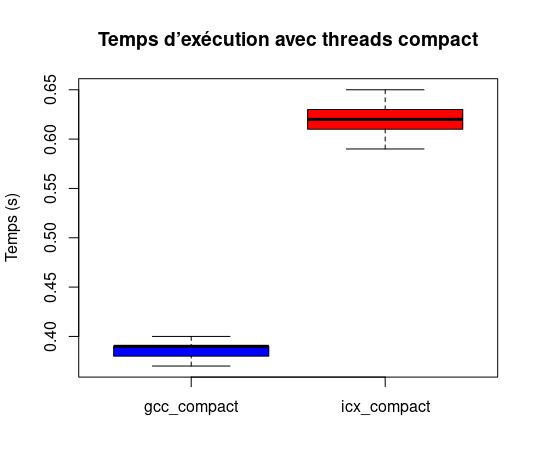
\includegraphics[width=0.5\textwidth]{../benhmark/compact.png}
                %\caption{}
                %\label{fig:compact}
            \end{figure}

            On remarque que pour des threads placés de manière rapproché, \textit{gcc} est une nouvelle fois plus performant que \textit{icx}. On a un intervalle de données restreint, allant de 0,37 à 0,41 pour \textit{gcc} et de 0,59 à 0,65 pour \textit{icx}.
        \subsection{Threads scatter}
        Ici le placement des threads se fait manuellement grâce au script.
        \newline
        Voici les résultats obtenus pour les exécutions avec threads éloignés :

        \begin{figure}[H]
            \centering
            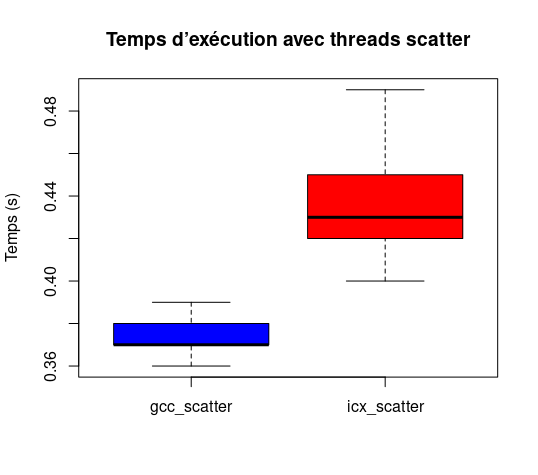
\includegraphics[width=0.5\textwidth]{../benhmark/scatter.png}
            %\caption{}
            %\label{fig:scatter}
        \end{figure}

        On remarque que pour des threads placés de manière éloigné, \textit{gcc} est une nouvelle fois plus performant que \textit{icx}. On a un intervalle de données allant de 0, 35 à 0,40 pour \textit{gcc} et de 0,40 à 0,52 pour \textit{icx}.
    \clearpage
    \part{Conclusion}
    Durant ce TP, nous avons étudié l'importance des placements de threads pour améliorer les performances de notre programme. Nous avons, pour cela, exploré trois types de placements de threads : 
    \newline \indent
        Le placement de threads dit sans affinité : Ici c'est l'OS qui place les threads automatiquement. Les résultats obtenus ont montré une grande diversité de temps de part le grand intervalle de valeurs générés. L'avantage de ce placement est que l'OS s'occupe de tout mais cette méthode peut être inefficace en termes d'utilisation du cache car les threads peuvent être déplacés d'un cœur à un autre au cours de l'exécution, ce qui explique le grand intervalle de données.
        \newline \indent
        Le placement de threads compact : On assigne volontairement des threads à des cœurs proches les uns des autres pour un partage du cache. Cette méthode permet un partage du cache plus efficace et donc d'améliorer la communication entre les threads, ce qui réduit le temps d'exécution. On le confirme avec les résultats obtenus, l'intervalle de données étant petit. Les inconvénients ici sont la saturation du cache et la sous-utilisation des autres cœurs.
        \newline \indent
        Le placement de threads scatter : On placement les threads sur des cœurs éloignés les uns des autres. Cela permet au thread d'avoir un accès dédié au cache, réduisant les interférences entre les threads. Utile pour les applications qui ne partagent pas les même données. Cela peut également augmenter la latence de communication entre les threads s'il y a des dépendances de données entre les eux.
        \newline
        \indent
        En résumé, il est nécessaire d'étudier notre application en profondeur pour connaître les éventuelles dépendances de données pour placer nos threads en fonction des besoins.
\end{document}
